\chapter{Evaluación y validación de la herramienta}\label{cap:evaluacion}

Este capítulo presenta la evaluación de CloudPorter, orientada a comprobar que lo construido
funciona y que responde a los requisitos definidos en el capítulo~\ref{cap:especificacion}. Dado
que el trabajo se plantea como una prueba de concepto, la evaluación no persigue una verificación
exhaustiva de calidad, sino evidenciar que el enfoque es viable de extremo a extremo y que el
alcance comprometido para la versión inicial se ha alcanzado. A continuación se exponen los
objetivos de la evaluación, la metodología seguida, los escenarios considerados, los criterios de
éxito, los resultados obtenidos y una discusión de sus limitaciones.

\section{Objetivos de la evaluación}

La evaluación persigue dos objetivos complementarios. El primero es comprobar que CloudPorter
\textbf{cumple los requisitos} funcionales y no funcionales recogidos en el
capítulo~\ref{cap:especificacion}, que delimitan el alcance de la prueba de concepto. El segundo,
más cualitativo, es demostrar que la idea de fondo del trabajo —la \textbf{interoperabilidad} entre
proveedores— se materializa en la práctica: que una misma definición agnóstica puede traducirse y
desplegarse en distintas nubes sin reescribirla.

No se trata, por tanto, de una campaña de pruebas orientada a un producto cerrado, sino de aportar
la evidencia mínima necesaria para sostener que el enfoque funciona y que el subconjunto de
funcionalidades construido se comporta como se especificó.

\section{Metodología de evaluación}

La evaluación combina tres métodos complementarios, escogidos por su adecuación a una prueba de
concepto, donde lo relevante es demostrar viabilidad y cobertura del alcance antes que exhaustividad.

\begin{itemize}
    \item \textbf{Validación funcional frente a requisitos:} cada requisito funcional (RF) y no
    funcional (RNF) del capítulo~\ref{cap:especificacion} se contrasta con la funcionalidad
    realmente implementada, determinando si se cumple y en qué parte del desarrollo se materializa.

    \item \textbf{Despliegue real de extremo a extremo:} se valida el flujo completo —del Manifest
    a la infraestructura desplegada— ejecutándolo sobre \textbf{AWS} y \textbf{Microsoft Azure} a
    partir del mismo manifiesto, sin más cambio que el del proveedor de destino. Es la prueba
    directa de la interoperabilidad.

    \item \textbf{Suite de tests automatizados:} el comportamiento del código se respalda con una
    suite de pruebas con un umbral mínimo de cobertura del 80\,\%, exigido por la integración
    continua, que actúa como red de seguridad frente a regresiones a lo largo del desarrollo.
\end{itemize}

\section{Escenarios de prueba y casos de uso evaluados}

El escenario central de la evaluación es una \textbf{aplicación de inventario de tres capas}, que
integra todas las capacidades de la herramienta en un caso realista. La aplicación se compone de un
frontend servido con nginx, un backend en Node.js con Express y una base de datos MySQL gestionada,
descritos en un \textbf{único manifiesto}. Este caso es significativo porque ejercita de forma
conjunta la traducción de cómputo y de base de datos, la red autogenerada, la exposición pública,
los scripts de arranque y las referencias entre recursos, y porque se despliega en ambos
proveedores cambiando solo el argumento \texttt{--provider}.

De forma complementaria, el \href{https://github.com/lucpez/cloudporter/tree/main/examples}{directorio de ejemplos del proyecto} incluye \textbf{manifiestos
mínimos} que aíslan cada funcionalidad —un recurso de cómputo, una base de datos, un recurso
público con script de arranque— y que permiten validar cada pieza por separado antes de combinarlas.

El recorrido detallado de la demostración, paso a paso, se recoge en el anexo de manual de uso, con
el fin de no mezclar aquí la validación con el tutorial.

\section{Métricas y criterios de evaluación}

Al tratarse de una prueba de concepto, los criterios de éxito son fundamentalmente cualitativos y
binarios —la capacidad funciona o no—, complementados con un único umbral cuantitativo sobre la
cobertura de pruebas. Se consideran satisfactorios los siguientes criterios:

\begin{itemize}
    \item \textbf{Traducción correcta y determinista:} el mismo manifiesto produce siempre las
    mismas plantillas de OpenTofu, válidas para cada proveedor.

    \item \textbf{Despliegue de extremo a extremo:} la infraestructura se despliega correctamente
    en AWS y en Azure desde la misma definición, y la aplicación resulta accesible.

    \item \textbf{Comparativa de costes coherente:} el comando \texttt{estimate} produce una
    estimación comparable entre proveedores antes del despliegue.

    \item \textbf{Detección de anti-patrones:} el comando \texttt{audit} identifica configuraciones
    arquitectónicas inseguras en el manifiesto.

    \item \textbf{Cobertura de pruebas:} la suite de tests supera el umbral del 80\,\% exigido por
    la integración continua.

    \item \textbf{Cobertura de requisitos:} los requisitos funcionales y no funcionales del
    capítulo~\ref{cap:especificacion} quedan satisfechos.
\end{itemize}

\section{Resultados obtenidos}

\subsection*{Validación frente a los requisitos}

La tabla~\ref{tab:validacion-rf} resume el grado de cumplimiento de los requisitos funcionales y la
tabla~\ref{tab:validacion-rnf} el de los no funcionales, indicando en cada caso la iteración del
capítulo~\ref{cap:desarrollo} en la que se materializan. Todos los requisitos definidos para la
versión inicial se han satisfecho.

\begin{table}[H]
\centering
\begin{tabular}{llp{6.2cm}}
\hline
\textbf{Requisito} & \textbf{Estado} & \textbf{Evidencia} \\
\hline
RF-01. Manifest YAML agnóstico      & Cumplido & Iteración 1 (definición del manifiesto) \\
RF-02. Validación del Manifest      & Cumplido & Iteración 1 (comando \texttt{validate}) \\
RF-03. Traducción a OpenTofu        & Cumplido & Iteraciones 2 y 4 (AWS y Azure) \\
RF-04. Cómputo, BD y red            & Cumplido & Iteraciones 2, 4 y 6 \\
RF-05. Mapper determinista          & Cumplido & Iteraciones 2 y 4 \\
RF-06. Despliegue                   & Cumplido & Iteración 3 (comando \texttt{deploy}) \\
RF-07. Estado del despliegue        & Cumplido & Iteración 3 (resumen de recursos) \\
RF-08. Estimación de costes         & Cumplido & Iteración 5 (comando \texttt{estimate}) \\
RF-09. Comparativa entre proveedores& Cumplido & Iteración 5 \\
RF-10. Interfaz de línea de comandos& Cumplido & Iteraciones 1, 3 y 5 \\
RF-11. Análisis de seguridad        & Cumplido & Iteración 7 (comando \texttt{audit}) \\
\hline
\end{tabular}
\caption{Validación de los requisitos funcionales frente a lo implementado.}
\label{tab:validacion-rf}
\end{table}

\begin{table}[H]
\centering
\begin{tabular}{llp{6.2cm}}
\hline
\textbf{Requisito} & \textbf{Estado} & \textbf{Evidencia} \\
\hline
RNF-01. Determinismo    & Cumplido & Traducción sin componentes aleatorios ni APIs externas \\
RNF-02. Extensibilidad  & Cumplido & Carga dinámica de módulos por proveedor \\
RNF-03. Usabilidad      & Cumplido & El usuario opera en términos del Manifest \\
RNF-04. Trazabilidad    & Cumplido & \texttt{translate} expone las plantillas antes de desplegar \\
RNF-05. Mantenibilidad  & Cumplido & Estructura en capas orquestador-proveedor-recurso \\
\hline
\end{tabular}
\caption{Validación de los requisitos no funcionales frente a lo implementado.}
\label{tab:validacion-rnf}
\end{table}

\subsection*{Despliegue de extremo a extremo}

El caso de la aplicación de tres capas se desplegó con éxito sobre AWS y sobre Azure a partir del
mismo manifiesto, sin más diferencia que el proveedor seleccionado, y la aplicación quedó accesible
en ambos casos, como muestran las figuras~\ref{fig:demo-aws} y~\ref{fig:demo-azure}. Que la misma
definición resulte funcional en dos nubes distintas, sin reescribir una sola línea, constituye la
evidencia central de la interoperabilidad que persigue el trabajo.

\begin{figure}[H]
\centering
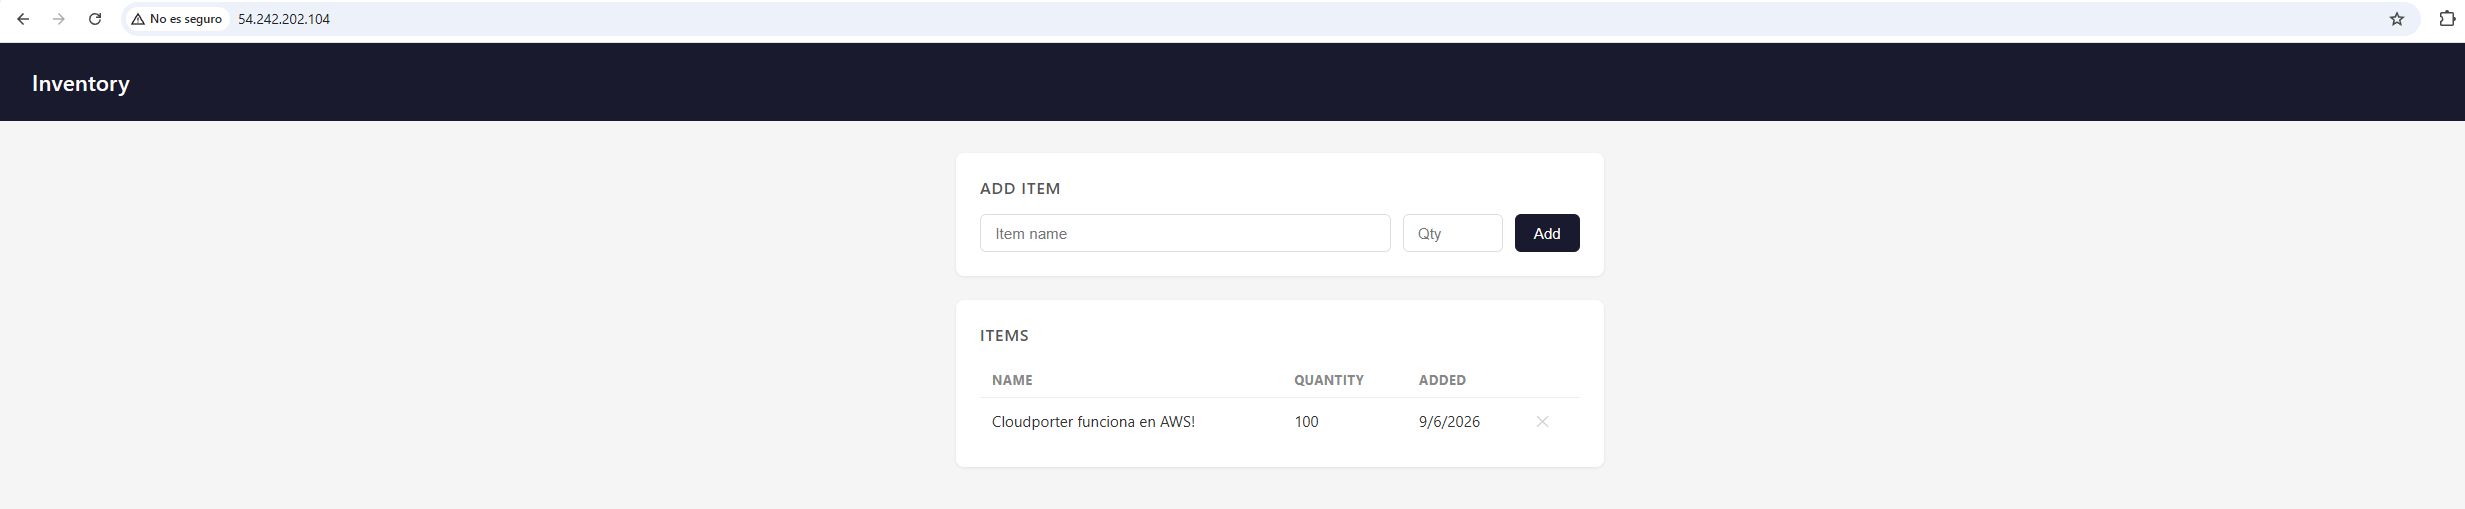
\includegraphics[width=\textwidth]{figures/inventory_app_works_in_aws.png}
\caption{Aplicación de inventario en funcionamiento tras desplegarse en \textbf{AWS} desde el manifiesto.}
\label{fig:demo-aws}
\end{figure}

\begin{figure}[H]
\centering
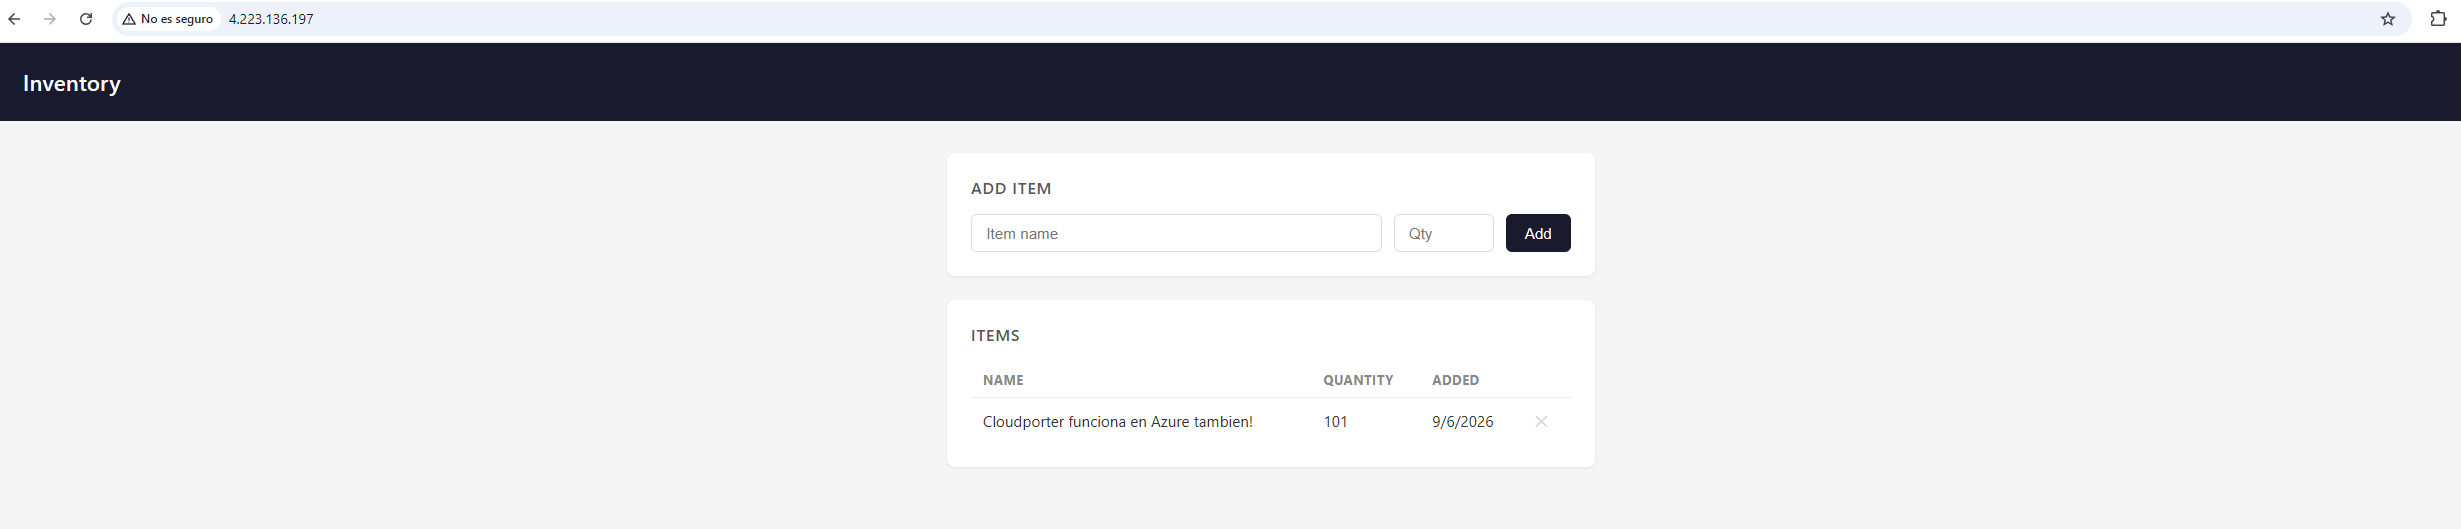
\includegraphics[width=\textwidth]{figures/inventory_app_works_in_azure.png}
\caption{La misma aplicación, desplegada en \textbf{Azure} con el mismo manifiesto sin más cambio que el proveedor.}
\label{fig:demo-azure}
\end{figure}

\subsection*{Estimación de costes y auditoría}

El comando \texttt{estimate} produce una comparativa de coste mensual entre proveedores antes de
desplegar, como muestra el extracto de código~\ref{lst:estimate}, lo que permite fundamentar la
elección de proveedor en criterios económicos. Por su parte, el comando \texttt{audit} detecta
anti-patrones arquitectónicos sobre el propio manifiesto; el extracto de
código~\ref{lst:audit} recoge la advertencia emitida ante una base de datos sin una capa de cómputo
que actúe como capa de aplicación.

\subsection*{Cobertura de pruebas}

La \href{https://github.com/lucpez/cloudporter/tree/main/tests}{suite de tests automatizados} alcanzó una cobertura del 86\,\%, por encima del umbral mínimo del
80\,\% exigido por la integración continua en cada cambio, como recoge la figura~\ref{fig:cobertura}.
No se persiguió la cobertura total. 

La fracción no cubierta corresponde, principalmente, al código
que interactúa con sistemas externos —la invocación de OpenTofu y de las APIs de los proveedores
cloud, que la suite sustituye por \textit{mocks} para ejecutarse de forma rápida, determinista y sin
incurrir en coste— y a algunos casos límite de esa interacción. Esos caminos quedan fuera de las
pruebas automatizadas, pero no sin validar: su correcto funcionamiento se comprobó de forma manual,
mediante los despliegues reales sobre AWS y Azure descritos al inicio de esta sección. Las pruebas
unitarias validan así la lógica, mientras que los despliegues manuales confirman la integración con
la nube.

Una mejora futura sería sistematizar esa comprobación con una suite de pruebas de extremo a extremo
que ejecute despliegues reales, en lugar de sustituir esa interacción por \textit{mocks} como hace la
suite unitaria actual. Esta y otras líneas de mejora se desarrollan en el
capítulo~\ref{cap:conclusiones}.

\begin{figure}[H]
\centering
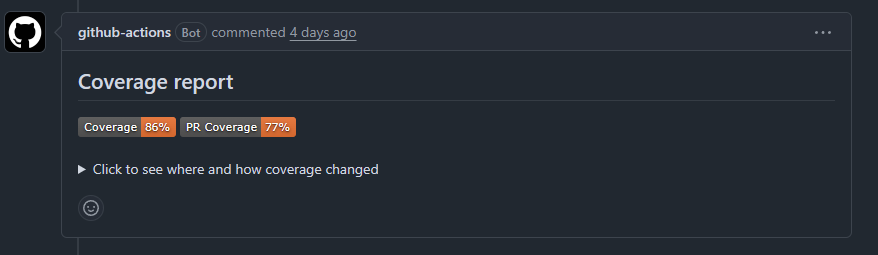
\includegraphics[width=0.65\textwidth]{figures/reporte_covertura_test_final.png}
\caption{Informe de cobertura de la suite de tests, publicado automáticamente por la integración continua en cada pull request.}
\label{fig:cobertura}
\end{figure}

\section{Discusión de resultados y limitaciones}

Los resultados anteriores sostienen las dos tesis de la evaluación. Por un lado, todos los
requisitos definidos para la versión inicial se cumplen. Por otro, la prueba más exigente —desplegar
una aplicación realista en dos nubes distintas desde una única definición— se supera, lo que valida
el enfoque de interoperabilidad como algo más que una propuesta teórica.

Conviene, no obstante, enmarcar estos resultados en el alcance de la propia evaluación, acorde con
el carácter de prueba de concepto del trabajo. La validación de extremo a extremo se concentra en un
único escenario de demostración, representativo pero no exhaustivo, y la integración con la nube se
comprueba mediante despliegues manuales, dado que la suite automatizada sustituye esa interacción por
\textit{mocks}, según se detalló en el apartado de cobertura. Son, por tanto, limitaciones de la
validación realizada, no del enfoque que esta valida.

Junto a ellas existen las limitaciones de alcance de lo construido —el subconjunto de proveedores,
tipos de recurso y servicios cubierto—, que no son objeto de este capítulo, sino del balance final:
se retoman y discuten en el capítulo~\ref{cap:conclusiones}.
